\documentclass[10pt,a4paper]{article}
\usepackage[bindingoffset=0.2in,%
            left=2.5cm,right=2cm,top=2.7cm,bottom=1in,%
            footskip=.25in]{geometry}
\usepackage[utf8]{inputenc}
\usepackage[ngerman]{babel}
\usepackage{amsmath, amsfonts, amssymb}
\usepackage{scrpage2}
\usepackage{color}
\usepackage{titlesec}
\pagestyle{scrheadings}
\usepackage{ulem, contour}
\usepackage{multicol}
\usepackage{hyperref}
\usepackage{pdfpages}
\usepackage{tabularx}
\usepackage{subcaption}
\usepackage{scrextend}
\usepackage{enumerate, enumitem}
\usepackage[bottom, splitrule]{footmisc}
\usepackage{multirow}
\usepackage{csquotes}
\usepackage{minted}

\usepackage[style=authoryear, backend=biber]{biblatex}
\addbibresource{bibliography.bib}

\renewcommand{\ULdepth}{1.8pt}
\contourlength{0.8pt}

\newcommand{\cul}[1]{%
  \uline{\phantom{#1}}%
  \llap{\contour{white}{#1}}%
}

\graphicspath{
    {Images/}
}

\makeatletter
\newcommand*{\rom}[1]{\expandafter\@slowromancap\romannumeral #1@}
\makeatother

\newrobustcmd*{\parentexttrack}[1]{%
  \begingroup
  \blx@blxinit
  \blx@setsfcodes
  \blx@bibopenparen#1\blx@bibcloseparen
  \endgroup}

\AtEveryCite{%
  \let\parentext=\parentexttrack%
  \let\bibopenparen=\bibopenbracket%
  \let\bibcloseparen=\bibclosebracket}

\definecolor{gray}{rgb}{0.33, 0.33, 0.33}
\definecolor{greengreen}{rgb}{0.0, 0.56, 0.0}
\definecolor{fgreen}{rgb}{0.13, 0.55, 0.13}
\definecolor{grellow}{rgb}{0.68, 1.0, 0.18}
\definecolor{orange}{rgb}{1.0, 0.49, 0.0}
\definecolor{deepblue}{rgb}{0,0,0.5}
\definecolor{deepred}{rgb}{0.6,0,0}
\definecolor{deepgreen}{rgb}{0,0.5,0}

\usepackage{pifont}

\newcommand{\cmark}{\ding{51}}%
\newcommand{\xmark}{\ding{55}}%
\newcommand{\wontfix}{\rlap{$\square$}{\large\hspace{1pt}\xmark}}


\newcommand{\vnr}{2}
\newcommand{\anr}{1}

\ihead{}
\ohead{Anfängerpraktikum 2}
\chead{Versuch \vnr, Abgabe \anr : Messung von Widerständen}
\cfoot{\pagemark}
\setheadsepline{.5pt}
\setlength\parindent{0pt}

\begin{document}

\begin{multicols}{2}
\begin{labeling}{Versuch-Nr.:}
\item[\textcolor{white}{x}Protokollant:\hspace{38pt}] \cul{Name} \wontfix
\item[\textcolor{white}{x}Zusammenarbeit mit:] \cul{Name} $\square$
\item[\textcolor{white}{x}Datum:\hspace{62pt}] \cul{\today}

\columnbreak

\item[Kurs: \hspace{27pt}] \cul{Anfängerpraktikum 2}
\item[Assistent: \hspace{8.7pt}] \cul{Name}
\item[Versuch-Nr.:] \underline{\vnr}
\end{labeling}
\end{multicols}

\begin{figure}[h]
\hspace{-0.5cm}\centerline{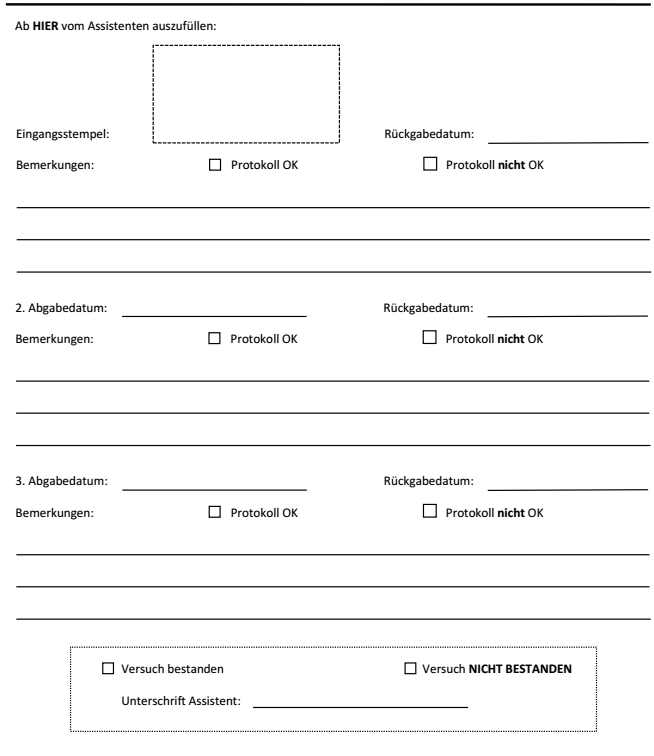
\includegraphics[width=1.1\linewidth , height=19cm]{Deckblatt_rest}}
\end{figure}

\newpage

\tableofcontents

\vspace{10pt}

\section{Aufgabenstellung}
\begin{flushleft}
Der Versuch \vnr behandelt das Messen von Widerständen im Einzelnen, in Reihen- und in Parallelschaltung sowie das Messen des Widerstandes an einer Lampe.
\end{flushleft}

\subsection{Physikalischer Hintergrund}
\begin{flushleft}
Zwischen Strom, Spannung und Widerstand besteht der Zusammenhang der \textit{URI}-Formel:
\begin{equation}\label{eq:uri}
U = R \cdot I
\end{equation}
Zusätzlich existiert der sog. \textit{spezifische Widerstand}:
\begin{equation}\label{eq:spezwi}
R = \rho \cdot \frac{l}{A}
\end{equation}
\end{flushleft}

\section{Messmethoden}
\begin{flushleft}
Wir messen den Strom und die Spannung an den Widerständen mit Volt- und Amperemeter.
\end{flushleft}

\subsection{Versuchsaufbau}
\begin{flushleft}
Für diesen Versuch benötigen wir:
\begin{itemize}[itemsep=0pt]
\item Zwei Widerstände (unbekannter Größe)\footnote{Widerstand $R_1$ soll dabei ein Draht mit Länge $l = 303cm$ und Quersschnittsfläche $A = 2.5mm^2$ sein.}
\item Eine Lampe (230V, 60W)
\item Ein Voltmeter zum messen der Spannung
\item Ein Amperemeter zum messen des Stromes
\end{itemize}
Alternativ zu Volt- und Amperemeter können auch Multimeter eingesetzt werden.
\end{flushleft}

\newpage

\subsection{Schaltpläne}
\begin{flushleft}
\begin{figure}[H]
\centering
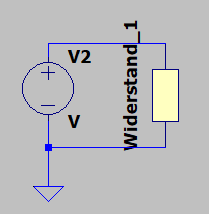
\includegraphics[scale=0.5]{schaltbild}
\caption{Schaltbild.}
\label{fig:schalt}
\end{figure}
Das Schaltbild (Abbildung \ref{fig:schalt}) zeigt den Aufbau für Widerstand 1. Für Widerstand 2, sowie die Reihen- und Parallelschaltung und die Lampe erfolgt die Schaltung analog.
\end{flushleft}

\section{Versuchsdurchführung}
\begin{flushleft}
Wir bauen die Schaltung (Abbildung \ref{fig:schalt}) auf und messen Strom- und Spannung. Anschließend schließen wir den Widerstand 2, eine Parallel- und danach eine Reihenschaltung der Widerstände an. Hier tragen wir die Spannung in Abhängigkeit des Stromes auf. Anschließend messen wir an der Lampe und tragen Widerstand in Abhängigkeit der Spannung auf.
\end{flushleft}

\section{Versuchsergebnisse}
\begin{flushleft}
Wir tragen die Messergebnisse in einem Graphen auf und bestimmen die Steigung des Graphen (Strom auf der X-Achse, Spannung auf der Y-Achse; Siehe auch: \ref{eq:uri}).
\begin{figure}[H]
\centering
\begin{subfigure}[c]{.5\textwidth}
\centering
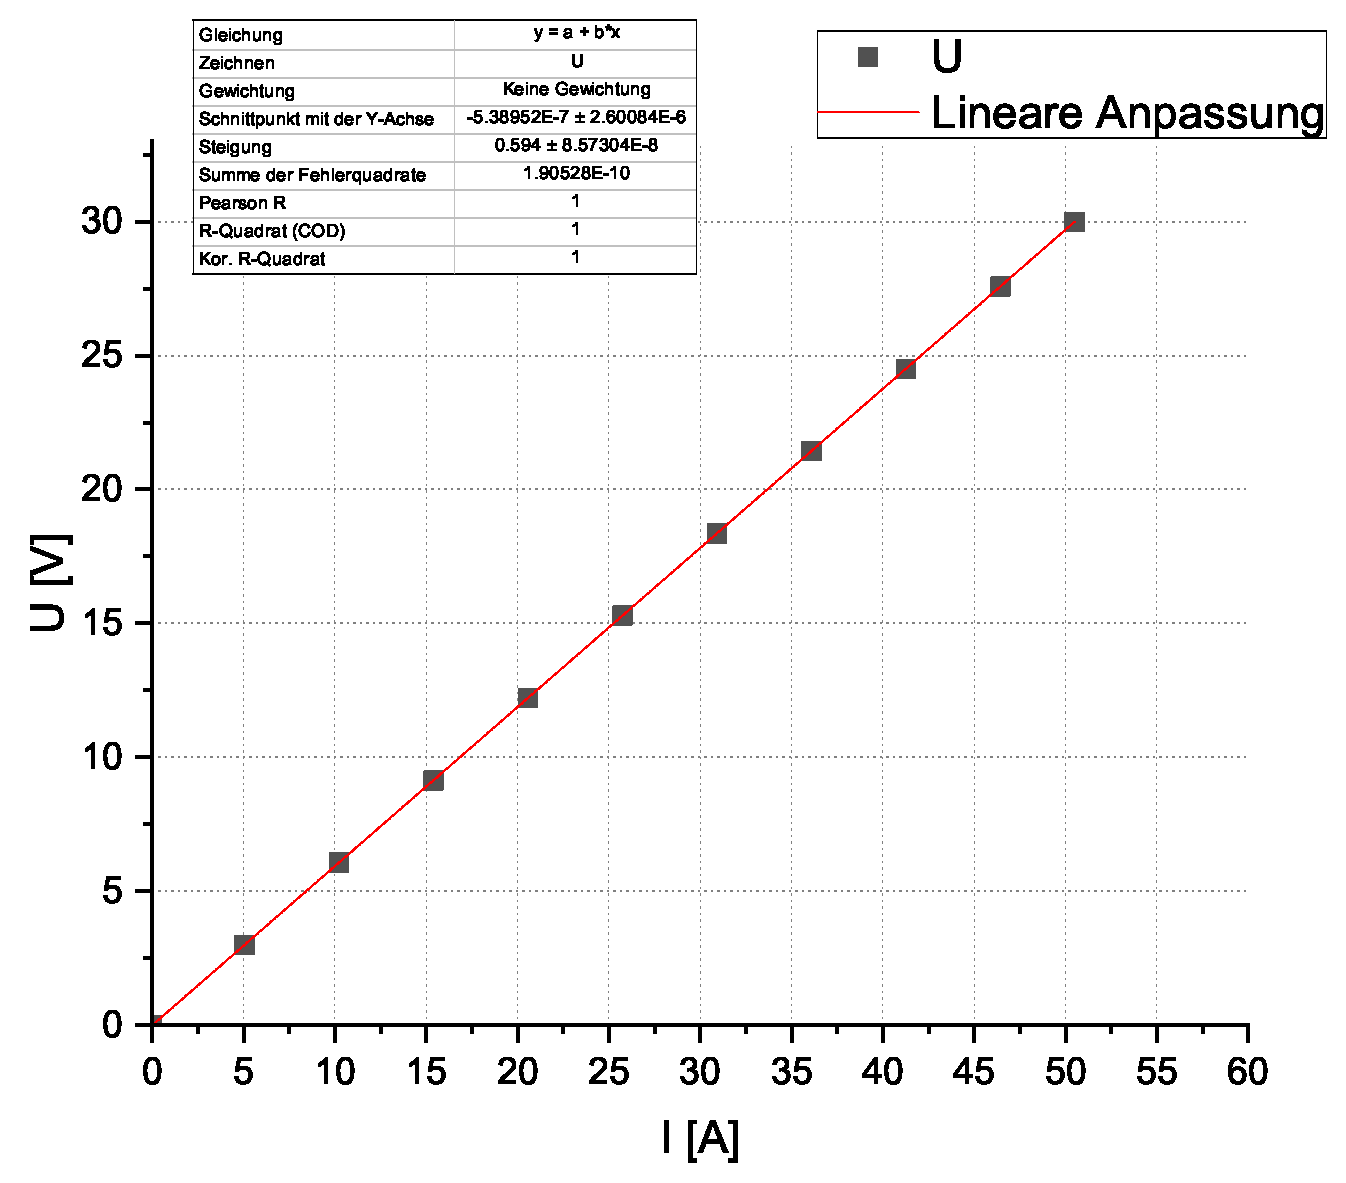
\includegraphics[scale=0.25]{R1}
\subcaption{Widerstand $R_1$}
\label{fig:r1}
\end{subfigure}%
%
\begin{subfigure}[c]{.5\textwidth}
\centering
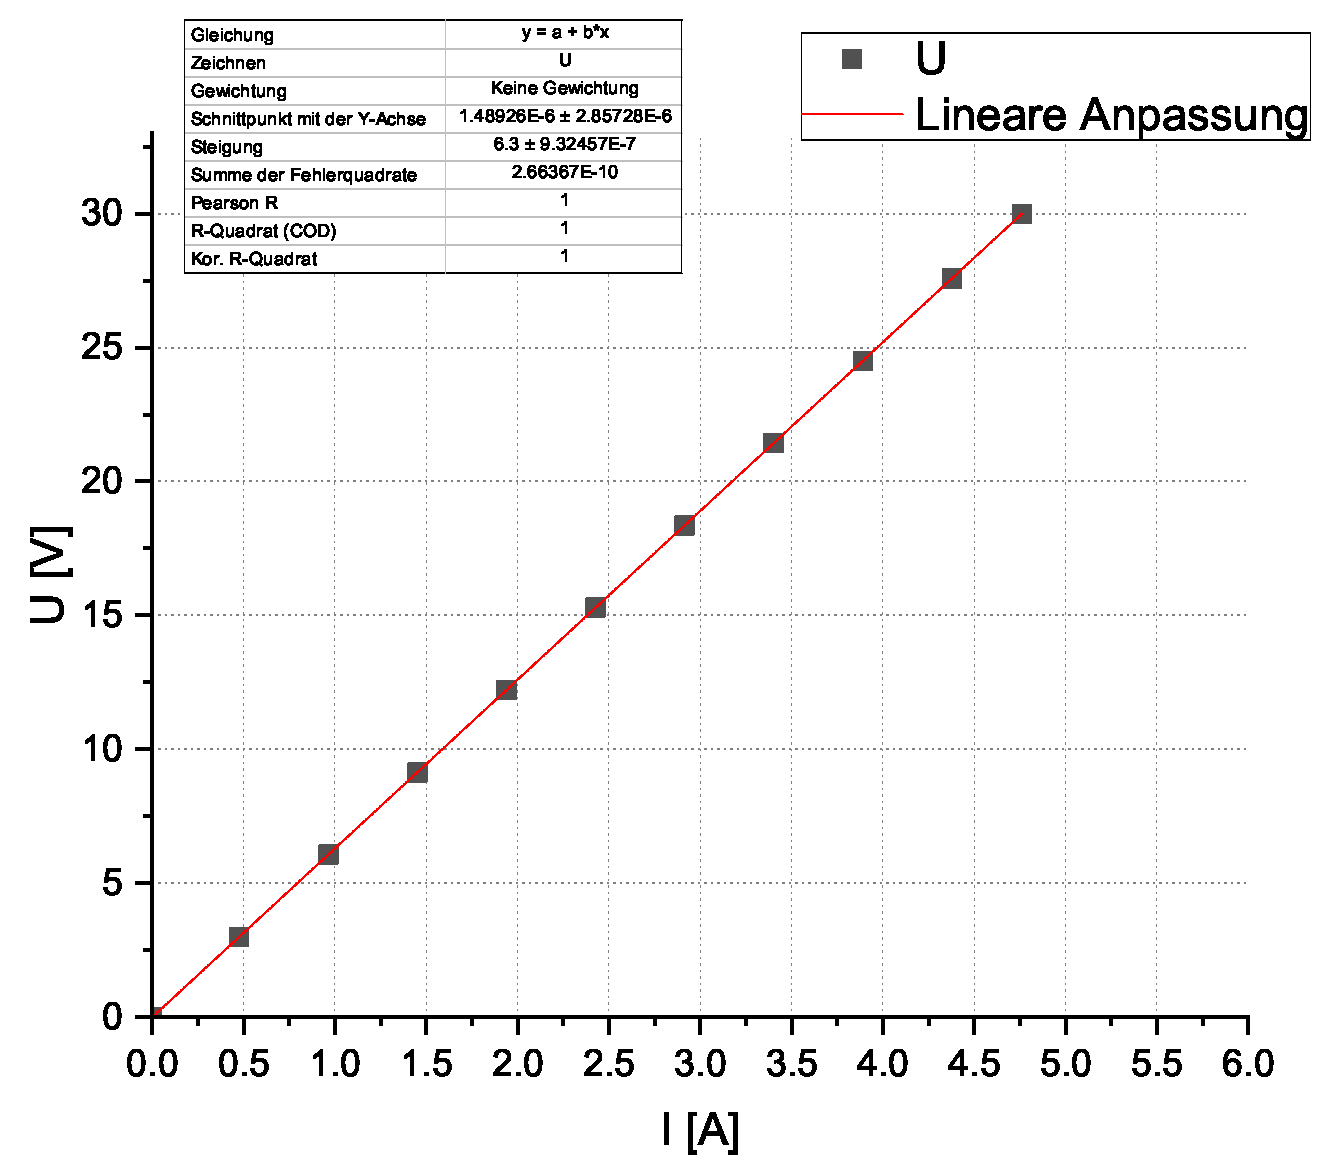
\includegraphics[scale=0.25]{R2}
\subcaption{Widerstand $R_2$}
\label{fig:r2}
\end{subfigure}%

\begin{subfigure}[c]{.5\textwidth}
\centering
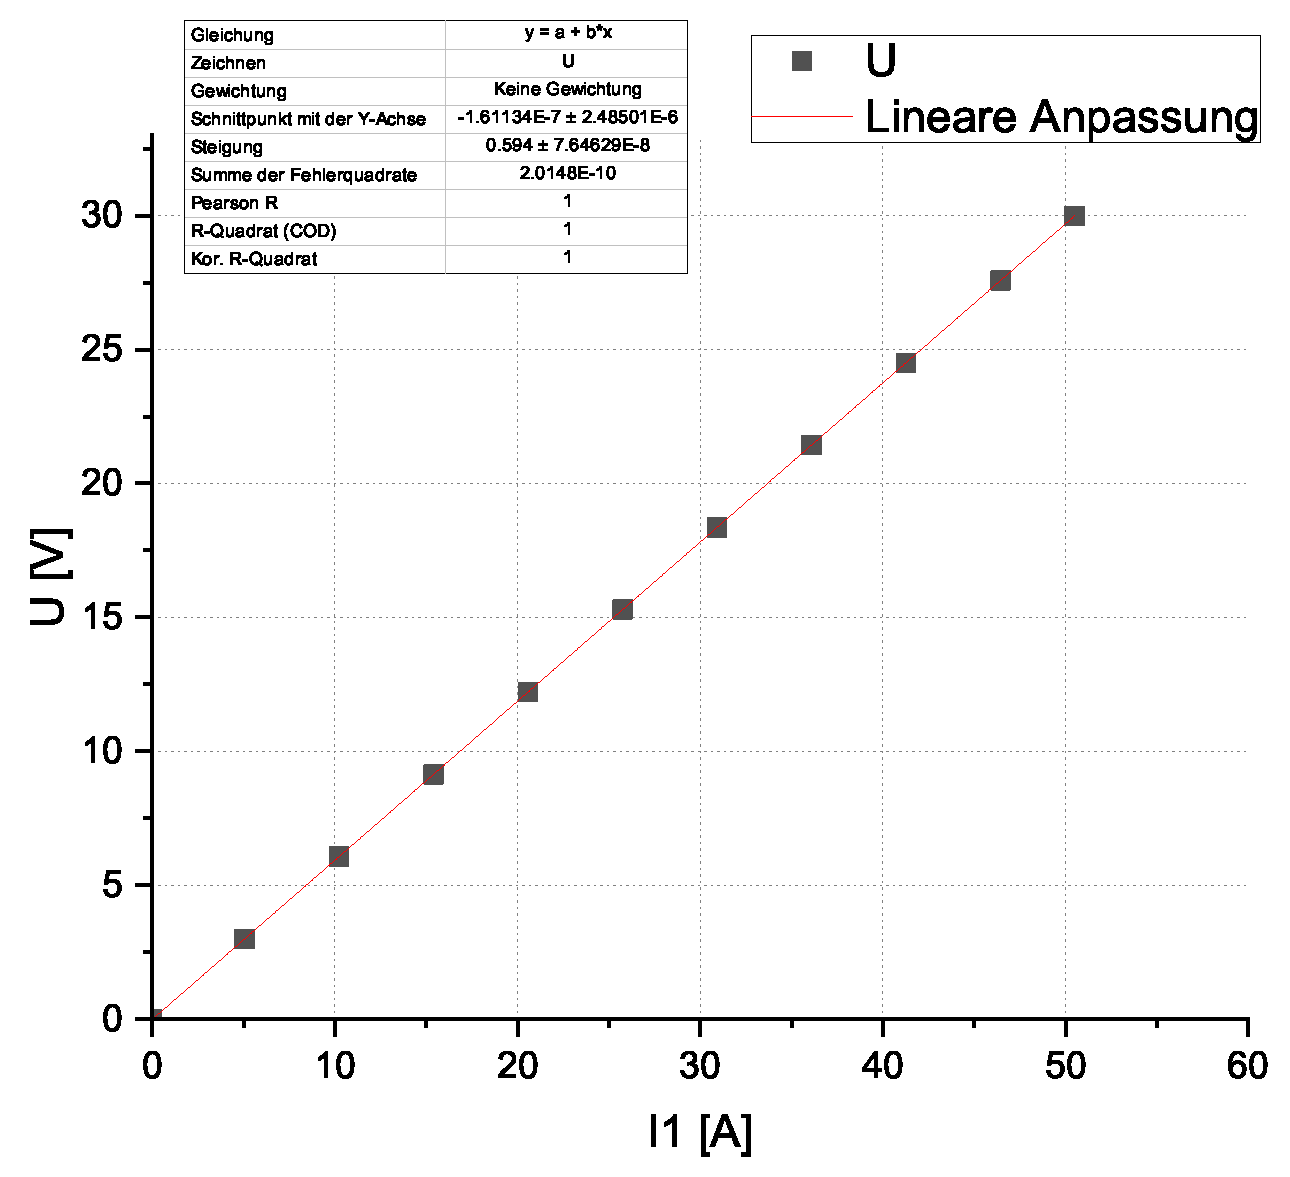
\includegraphics[scale=0.25]{Rpara}
\subcaption{Widerstand $R_{\parallel}$}
\label{fig:rpara}
\end{subfigure}%
%
\begin{subfigure}[c]{.5\textwidth}
\centering
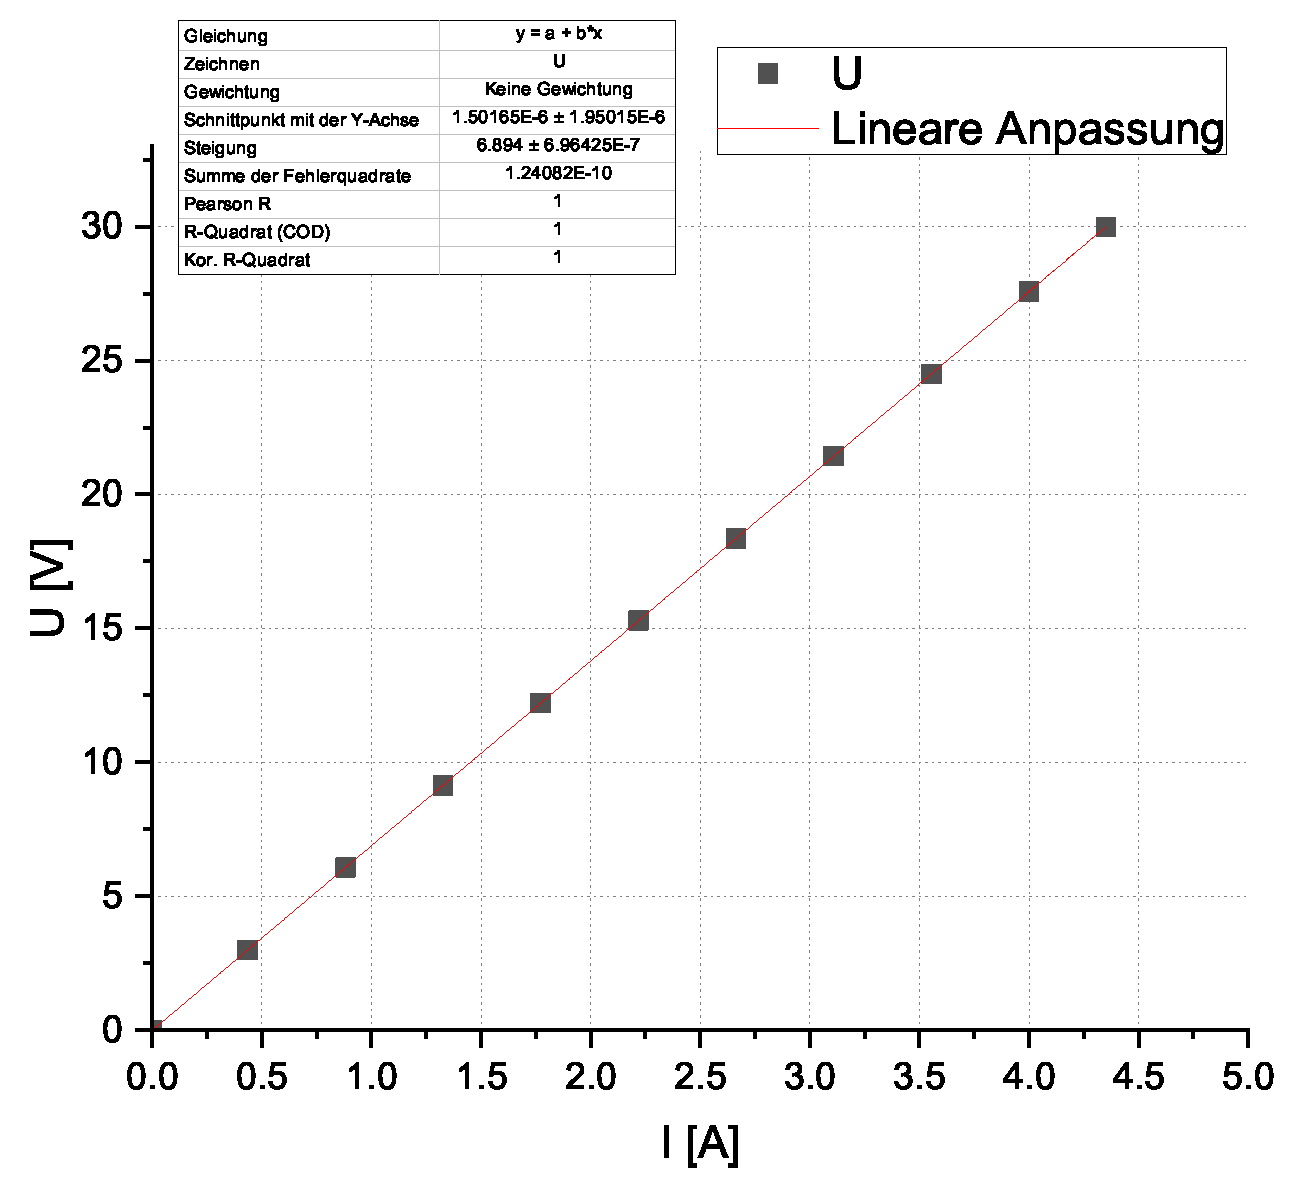
\includegraphics[scale=0.25]{Rreihe}
\subcaption{Widerstand $R_{\mid}$}
\label{fig:rreihe}
\end{subfigure}%
\caption{Widerstände 1 \& 2.}
\label{fig:wids}
\end{figure}
Wir haben also die Widerstände ermittelt:
\begin{align*}
R_1 &\approx (0.594 \pm 8.573 \cdot 10^{-8}) \Omega & R_2 &\approx (6.3 \pm 9.325 \cdot 10^{-7}) \Omega \\
R_{\parallel} &\approx (0.594 \pm 7.646 \cdot 10^{-8}) \Omega & R_{\mid} &\approx (6.894 \pm 6.964 \cdot 10^{-7}) \Omega
\end{align*}

\begin{figure}[H]
\centering
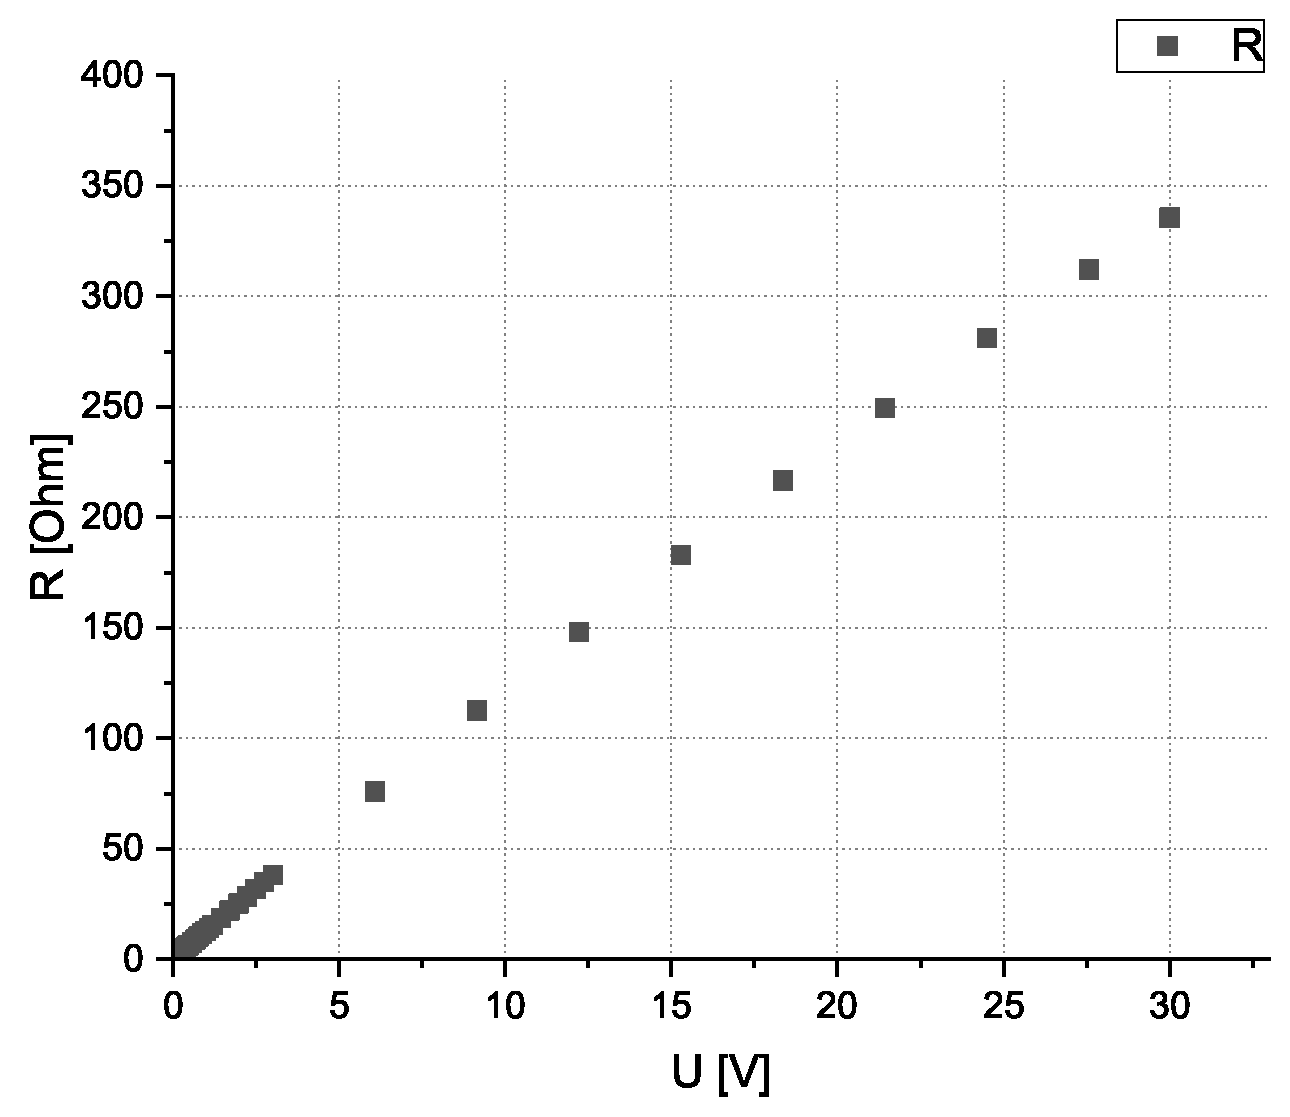
\includegraphics[scale=0.3]{Lampe}
\caption{Widerstand $R_{\otimes}$}
\label{fig:glampe}
\end{figure}
\end{flushleft}

\subsection{Diskussion der Messergebnisse}
\begin{flushleft}
\textbf{Widerstände $R_1$ udn $R_2$}

Die Graphen (Abbildung \ref{fig:wids}) zeigen, dass die Spannung proportional zur Spannung wächst.

Wir wollen nun noch den \textit{spezifischen Widerstand} von Widerstand $R_1$ berechnen. Dazu nutzen wir Gleichung \ref{eq:spezwi} und können in diese Formeln unsere bekannten Größen einsetzen.
\begin{equation*}
\rho = R \cdot \frac{A}{l} = 0.594 \cdot \frac{2.5 \cdot 10^{-6}m^2}{3.03m} \approx 8.251 \cdot 10^{-7} \Omega m \approx 0.8251 \mu \Omega m
\end{equation*}
Wir haben somit den \textit{spezifischen Widerstand} von $R_1$ berechnet. Der Wert beträgt $4.9 \mu \Omega m$.

Dieser Wert für den spezifischen Widerstand lässt darauf schließen, dass der Widerstand aus dem Material \textbf{Konstantan}\footnote{Quelle: \href{https://de.wikipedia.org/wiki/Spezifischer_Widerstand}{Wikipedia}} besteht. Dieses besitzt einen spezifischen Widerstand von $\rho_K = 5 \cdot10^{-1} \Omega \frac{mm^2}{m}$ und weicht somit nur um $1 \cdot 10^{-2}$ von dem berechneten Wert ab\footnote{Umrechnung: $4.9 \mu \Omega m = 0.49 \Omega \frac{mm^2}{m}$}.
\end{flushleft}
\begin{flushleft}
\textbf{Lampe}

Der Graph zur Lampe (Abbildung \ref{fig:glampe}) zeigt, dass der Widerstand nicht ganz linear mit der Spannugn anwächst, der Verlauf ist leicht gekrümmt. \\

\textit{Vergleich des Maximalwiderstandes mit den Kenndaten}:

Aus dem Graphen ist zu entnehmen, dass der Maximalwiderstand $R_{max} \approx 340 \Omega$ besitzt.

Mit den Kenndaten der Lampe können wir den Widerstand der Lampe bestimmen:
\begin{align*}
P &= U \cdot I = U \cdot \frac{U}{R} \\
R &= \frac{U^2}{P} \\
&= \frac{(230 V)^2}{60W} \approx 881.667 \Omega
\end{align*}
Die Lampe hat in unserem Versuch somit weniger als die Hälfte des Kenndatenwiderstandes erreicht.
\end{flushleft}

\section{Fazit}
\begin{flushleft}
Der Versuch \vnr hat das Verhalten von Widerständen zu Strom- und Spannung näher beleuchtet udn gezeigt, dass die Linearität in der Realität bei Alltagsgegenständen nicht immer eingehalten ist.
\end{flushleft}

\begingroup
\raggedright
\sloppy
\printbibliography[heading=bibintoc,title={6 \hspace{6pt} Literatur}]
\endgroup

\end{document}